\documentclass[a4paper]{article}

\usepackage[utf8]{inputenc}
\usepackage[portuges]{babel}
\usepackage{indentfirst}
\usepackage{graphicx}

\title{Projeto de Laboratórios de Informática 3\\Grupo 21}
\author{Diogo Braga A82547 \and João Silva A82005 \and Ricardo Caçador A81064}
\date{\today}

\begin{document}

\maketitle

\begin{abstract}
  Este documento apresenta o projeto de Laboratórios de Informática
  3 (LI3), do curso de Engenharia Informática da Universidade
  do Minho.

  O projeto baseia-se na criação de um sistema de análise de ficheiros 
  XML que possuem informações do Stack Overflow, um website de perguntas
  e respostas sobre programação de computadores.

\end{abstract}

\tableofcontents
\listoffigures

\section{Introdução}
\label{sec:intro}

Este documento apresenta uma possível estrutura para o relatório da 2ª
fase do projeto da disciplina de Laboratórios de Informática 1 (LI1),
da Licenciatura em Engenharia Informática da Universidade do Minho,
que toma a forma de um projeto de média dimensão a ser desenvolvido na
linguagem de programação funcional Haskell.

Nesse contexto, este relatório deve relatar o trabalho desenvolvido
pelos alunos para atingir o resultado final nesse projeto, devendo
acompanhar a submissão da solução implementada. Além de servir de
treino das capacidades de comunicação escrita dos estudantes, servirá
também como elemento de avaliação para a utilização de \LaTeX{} pelos
alunos. Sendo assim o código fonte \LaTeX{} do relatório deve ser
mantido no repositório \texttt{svn} atribuído ao grupo\footnote{A
  ficha de LI1 dedicada ao \LaTeX{} disponibiliza informação técnica
  adicional sobre a utilização desta ferramenta.}. Um relatório desta
natureza tem geralmente uma dimensão entre 4 e 8 páginas, para além de
eventuais anexos.

A \emph{introdução} de um relatório apresenta de modo geral o trabalho
descrito no relatório: o problema que se pretende resolver, a sua
contextualização e a abordagem proposta pelos alunos para o
resolver. Deve passar ao leitor não só uma perspetiva geral do
trabalho desenvolvido mas também a motivação por trás dele.

Esta secção termina normalmente com uma apresentação da estrutura do
relatório, sendo aqui apresentada uma sugestão. Neste caso, a Secção
~\ref{sec:estruturas} apresenta as estruturas de dados utilizadas 
no projeto, a Secção~\ref{sec:estrategias} indica as estratégias usadas 
para resolver as  questões apresentadas, a Secção~\ref{sec:problema} descreve 
o problema a resolver enquanto a Secção~\ref{sec:solucao} apresenta e 
discute a solução proposta pelos alunos. O relatório termina com conclusões na
Secção~\ref{sec:conclusao}, onde é também apresentada uma análise
crítica dos resultados obtidos.


\section{Estruturas de Dados}
\label{sec:estruturas}

Esta secção tem as \emph{estruturas} do projeto.

\subsection{Estrutura TCD}
\begin{figure}[ht]
\centering
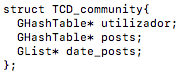
\includegraphics[scale=0.50]{image_tcd}
\caption{Estrutura TCD} 
\label{img:tcd}
\end{figure}

\subsection{Estrutura Utilizador}
\begin{figure}[ht]
\centering
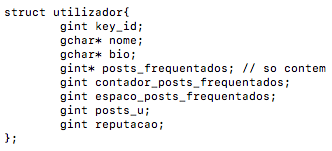
\includegraphics[scale=0.50]{image_utilizador}
\caption{Estrutura Utilizador} 
\label{img:utilizador}
\end{figure}

\subsection{Estrutura Posts}
\begin{figure}[ht]
\centering
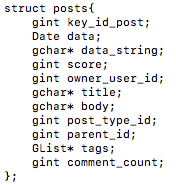
\includegraphics[scale=0.50]{image_posts}
\caption{Estrutura Posts} 
\label{img:posts}
\end{figure}


\section{Estratégias das Interrogações}
\label{sec:estrategias}

\subsection{Init}

\subsubsection{Melhoramento de Desempenho}

\subsection{Query 0}

\subsubsection{Melhoramento de Desempenho}

\subsection{Query 1}

Dado o identificador de um post, a função retorna o título do post 
e o nome de utilizador do autor. Se o post for uma resposta, a função
retorna o título e o id do utilizador da pergunta correspondente.

Nesta questão, sendo o valor do \textbf{id} igual ao da \textbf{key} 
da tabela de hash, recorremos à função da \textit{glib},
\textbf{g\_hash\_table\_lookup} que dado uma \textbf{key},
retorna o \textbf{value} associado. Caso nada seja encontrado,
é retornado NULL.

Tendo agora todos os valores referentes ao \textbf{post}, caso este
seja uma pergunta, é atríbuido à primeira coordenada o \textbf{title}
do post e à segunda o \textbf{nome} de quem realizou a questão.
Encontramos o \textbf{nome} do autor da questão invocando o parâmetro
\textbf{owner\_user\_id} na mesma função \textbf{lookup} utilizada 
anteriormente, passando agora a ser esse o \textbf{key/id} associado.

Caso seja uma resposta, o primeiro parâmetro é calculado usando a mesma 
função \textbf{g\_hash\_table\_lookup}, mas agora com o 
parâmetro \textbf{parent\_id}, que numa resposta retorna o \textbf{id} 
da pergunta ao qual esta respondeu. O segundo parâmetro é igualmente
calculado como se fosse uma pergunta, mudando apenas o novo 
\textbf{value} associado.

\subsubsection{Melhoramento de Desempenho}

\subsection{Query 2}

\subsubsection{Melhoramento de Desempenho}

\subsection{Query 3}

\subsubsection{Melhoramento de Desempenho}

\subsection{Query 4}

\subsubsection{Melhoramento de Desempenho}

\subsection{Query 5}

\subsubsection{Melhoramento de Desempenho}

\subsection{Query 6}

\subsubsection{Melhoramento de Desempenho}

\subsection{Query 7}

\subsubsection{Melhoramento de Desempenho}

\subsection{Query 8}

\subsubsection{Melhoramento de Desempenho}

\subsection{Query 9}

\subsubsection{Melhoramento de Desempenho}

\subsection{Query 10}

\subsubsection{Melhoramento de Desempenho}

\subsection{Query 11}

\subsubsection{Melhoramento de Desempenho}

\subsection{Clean}

\subsubsection{Melhoramento de Desempenho}


\section{Descrição do Problema}
\label{sec:problema}

Esta secção apresenta o \emph{problema} que se pretende resolver no
contexto do projeto de LI1 assim como o seu enquadramento, devendo
definir concretamente os objetivos que se pretendem atingir.

\section{Concepção da Solução}
\label{sec:solucao}

Esta secção deve descrever o trabalho efetivamente desenvolvido pelos
alunos para resolver o problema apresentado na secção
anterior. Segue-se uma sugestão de organização para esta secção.

\subsection{Estruturas de Dados}

Esta secção deve apresentar as \emph{estruturas de dados} mais
relevantes para a solução desenvolvida.

\subsection{Implementação}

Esta secção deve apresentar as soluções propostas pelos alunos para
atingir os objetivos propostos, assim como a sua \emph{implementação},
devendo também descrever os problemas encontrados e as decisões
tomadas para os ultrapassar. Apesar de poder conter excertos de código
fonte quando relevante, esta secção não deve servir como alternativa à
documentação do código fonte submetido.

\subsection{Testes}

Esta secção deve apresentar alguns dos \emph{testes} definidos pelos
alunos para testar as funcionalidades da solução desenvolvida.

\section{Conclusões}
\label{sec:conclusao}

A secção de \emph{conclusões} resume o restante documento, devendo
também apresentar uma análise crítica dos resultados atingidos tendo
em conta os objetivos definidos.

\end{document}